\chapter{Literature Review} \label{LiteratureReview}

The focus of this chapter is to analyse and breakdown current research and literature concerning the use of NLP models within a domain and their implementations, specifically looking into the area of academia. The domain for this research will be text classification on Student Feedback forms; NLP has many interconnecting domains, in which implementations can heavily affect performance and the returned results. As the theory behind NLP grows, it is vital to use the least computationally cost---effective methods in which this section will be looking at merging newer techniques with older models to potentially improve our understanding of NLP models.

\section{What is NLP?}

Fundamentally, Natural Language Processing is an area of Computer Science which enables computer systems to access and understand human linguistics \parencite{eisenstein2019introduction}, expanding, NLP is theoretically driven computation for the purpose of evaluating, interpreting, and depicting naturally occurring transcripts to a certain level of detail. Differing depths of linguistics are used for analysis in---order to return a desired human---like range of processing for a particular application (needs the cite).

Over the last 20 years, NLP has become an integral topic of Computer Science as it combines computational linguistics with a popular buzzword Artificial Intelligence or more accurately Machine Learning \parencite{ongsulee2017artificial}, these terms have been generalized as this area of computing heavily relies on theory from different departments. Human and machine communication mediums both have similarities, to which we can model our understandings on, syntax is an intrinsic value to both communications, and it is used to label every component of a language and its sets of rules \parencite{jain2018natural}.

The value of NLP is in its ability to remove ambiguity in linguistic forms, this explicitness results in a clear data---driven numeric structure for numerous types of applications \parencite{SAS2021NLP}. The returned data structures are a result of some form of input, NLP algorithms can handle speech, text, or images where of the appropriate architecture. The properties and potentials of NLP are now used for commercial spaces and for public interest, several areas including:

\begin{itemize}
    \item Machine Translation
    \item Speech Functions
    \item Dialog Interfaces
    \item Text Analysis
    \item Natural Language Generation
    \item Writing Assistance
\end{itemize}

The list above defines six key areas of NLP that are used in commercial spaces and majority appeal to the academic space; the listed six areas are a high---level overview at how different theoretical approaches combine in---order to perform a given task \parencite{dale2019nlp} for the purpose of this literature review, we will be looking at the most relevant areas in which aid this domain.

\section{Uses of NLP in Academic Institutions}

As NLP expands, so do its domains; a more recent use of NLP is within academic institutions. During the last term of a module, it is common for universities to collect data regarding its practices and teaching etiquette. Universities will utilize both formal and informal techniques for elicitation, typically a printed hand---copy or via an online questionnaire, thereafter student feedback is analysed to provide institutions with a gauge on how to improve students’ satisfaction, module content, structure, and teaching methods. Information elicitation is completed in the form of a survey, with two main question approaches, being “program---wide” and “module---specific” to target flexibility of opinion vs factual coverage \parencite{keane2005obtaining, beran2007s}.

During the academic year of 2019/2020, education became distanced due to COVID---19 and accordingly E---learning soared as academic institutes were forced to adapt their teaching mediums and operations to become temporality online only \parencite{burgess2020schools}, this resulted in a frequent uptake of online feedback. This surge of sudden online academia has resulted in rapid development of Massive Open Online Courses (MOOC), these E---learning platforms enable student feedback on an extensive scale with reputable data to develop and train NLP models \parencite{wang2021predicting}.

The data gathered is used to give insight if users are satisfied with their academic consumption, NLP methods can be applied to student feedback to give the academic institution an idea if its students are validating the unified theory of acceptance and use of technology (UTAUT) model \parencite{kayali2020adoption}. Large data sets such as a class of 200 students would be tedious and time consuming for a lecturer to manually analyse individual feedback; combining aspects of staff roles and deep learning would utilize the computational power required for sizeable datasets by minimizing the required engineering \parencite{lecun2015deep}.

Manual thematic analysis of a dataset to formulate codes and themes also allows for human error, poor judgement as interpretation is subjective, and themes may be overlooked \parencite{belotto2018data}. As more aspects of data---driven interactions between clientele can be applied to NLP, the development of an all---purpose, accurate and, secure method to automating the elicitation of necessary linguistic aspects from an input source is increasingly imperative \parencite{sindhu2019aspect}.

A generalised approach for analysing student feedback is with the use of Word Embedding, popular implementations are Word2Vec, GloVe \parencite{pennington2014glove}, and FastText \parencite{edalati2020potential}.

\section{Applicable Methods for Text Classification on Student Feedback}

The intended outcome is to evaluate student feedback surveys which will be targeted towards enhancing the level of learning and engagement by students; to achieve the desired results, the following techniques would be most suitable if appropriately applied in this context.

\subsection{Sentiment Analysis and Opinion Mining} The desired outcome is to derive subjective material from students’ input, this can be insights, discussions or opinions which automatically review the polarity (negative, neutral, or positive) of information regarding the academic facilities \parencite{kandhro2019student}. Sentiment Analysis has three levels of scope which can be reduced to emulate different levels of comprehension:

\begin{figure}[H]
    \centering
    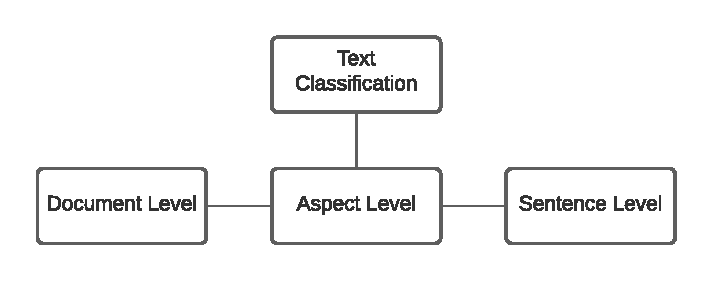
\includegraphics[width=\textwidth]{figures/chapter-2/TextClassificationTaxonomy.pdf}
    \caption[Taxonomical overview of Text Classification Levels]{Taxonomical overview of Text Classification Levels}
\end{figure}

\newpage

\textcite{kastrati2020weakly}, established an aspect---orientated opinion---mining model; student feedback was in English NL whereby three unique NLP techniques were applied to the dataset to produce three represented perceptions of the same dataset. The NLP techniques applied were: Word Embedding, Term Frequency (TF) and Term Frequency---Inverse Document Frequency (TF---IDF).

\textcite{kastrati2020weakly}, trained their models using already explored classifiers, Decision Tree, Naïve Bayes, Support Vector Machines and Boosted Graphs on a 1---Directional Convolutional Neural Network (1D---CNN). \textcite{kastrati2020weakly}, found traditional aspects of Machine Learning implementations yielded greater results than that of the sole use of a 1D---CNN.

\textcite{kastrati2020aspect} “Aspect---Based Opinion Mining of Students' Reviews” (2020) to produce a weakly supervised framework aimed at training deep learning models with little to no human interaction. Their proposed framework analyses a desired sentiment at document level and yielded an overall F1 score of 86.13\%  accuracy; they also tested their framework at the aspect level for SA to which yielded an F1 score of 82.1\%.

\subsection{Topic Labelling} This technique is used in conjunction with text mining to automatically handle significant and reoccurring themes and topics within students’ feedback with automatic creation of category labels per survey and section. LDA is a suitable model which can achieve the above, it uses Latent Dirichlet Distributions to group topics as a multinomial distribution of words and is able to associate words based on the probability distribution of the set \parencite{unankard2019topic}.

\subsection{Language Detection} This technique of NLP deals with determining which natural language (NL) is provided as the input source, this approach could be particularly beneficial to lecturers if the student and lecturer do not share the same first language; a classifier could be challenged by identifying an incorrect NL due to lexical and syntactical resemblance. These challenges could return pedagogical ambiguities within feedback \parencite{heift2017computer}, if a lecturer misinterprets student feedback due to a misunderstood lexical, an unintended impression will be represented.

This can be aided by converting NL structures in to a first---order logic (FOL) object to which these mathematical models will return the highest matching lexical in a percentage \parencite{perikos2017assistance}. Therefore, minimising miscommunication.

\subsection{Intent Detection} This technique is used to programmatically classify implied intent within an input, based on a certain ambition or outcome, usually a verbal adjective. Every student feedback survey has the same interaction purpose, to improve their quality of learning, this specific domain can be modelled to automatically categorise each intentional improvement specification. Intent classification can also be used to provide real---time feedback to lecturers opposed to standardised question---answer dialog systems \parencite{jensen2020toward}.

A common implementation of intent detection is with the use of a rule---based model, these systems use predefined constraints as intents with the hypothesis that occurring utterances conform with the predefined set of rules. These rules will be disputed when a novel utterance is parsed, as students have different methods of expressing their views, novel utterances will be frequent and with the appearance of utterances without a predefined label will increase, this problem exists under Zero---shot learning with CNNs \parencite{xia2018zero}.

However, textual classification is still an area of development and is not well---understood with regards to the most appropriate implementation, algorithm, and paradigm combination \parencite{thangaraj2018text}. An inherent objective of this paper will be looking at the amalgamations of theory to return the most effective and efficient results driven implementation for domain specific feedback classification.

\section{Related Research}

This section will predominantly concentrate on considerable studies of similar nature, these studies conduct research spotlighting technical performance of differing textual and contextual classification methods using different datasets and NLP models. Analysing previous literature will guide further development as they will give support towards vital features that are a prerequisite for essential system requirements, to the contrary, previous literature may outline features that are not of importance and potentially expose gaps in current research.

\subsection{Combination Classifiers}

The completed work in “a comparative study of classifier combination applied to NLP tasks” by \textcite{enriquez2013comparative}, was viewed as a comprehensive comparison and overview of diverging NLP implementations and combining methods for exercised NLP workloads. Enriquez and colleagues’ findings suggested lesser explored NLP models and classifiers yielded higher performance opposed to well---known implementations, for example, the combination of “stacking” anchors and “cascading” input layers for Part---of---Speech tagging returned results exceeding expectations \parencite{enriquez2013comparative}.

The fundamental concepts \textcite{enriquez2013comparative} encountered are applicable to modern development of combination classifiers; when developing a novel combination model, there are two compulsory criteria that must be met to be successful: heterogeneity of the chosen classifiers, this ensures a computational mistake will only be met once and will be provided a differing perception to an encountered error; veracity of the chosen classifiers, each classifier must reduce the occurrence of inaccuracies over another selected classifier.

An additional audit should be performed to verify the certainty of the desired classifiers will work together: statistical, are the chosen classifiers best suited? Given the problem based on previous resources; computational, accounting for time and space complexity, is there a potential to reach computational limits? That affect the desired result; representational, has the classifier been previously research to understand the objective task? Considering the criteria above, \textcite{enriquez2013comparative} chose to investigate:

\begin{itemize}
    \item Voting
    \item Bayesian Merging
    \item Behaviour Knowledge Space
    \item Bagging
    \item Stacking
    \item Feature Sub---spacing
    \item Cascading
\end{itemize}

The above NLP methods and techniques were applied to 9 different corpuses to train models for Part---of---Speech Tagging.

Since the work of \textcite{enriquez2013comparative}, NLP methods have advanced, more up---to---date findings reviewed in the paper “Prediction of Sentiment Analysis on Educational Data based on Deep Learning Approach” by \parencite{sultana2018prediction} centralises eight classifiers for performance inspection in which they are put against each other for speed, accuracy, and computational cost. This paper includes an open---sourced educational dataset from Kiteboard 360 which is provided to the individual classifiers, the classifiers tested were:

\begin{itemize}
    \item Support---Vector Machine (SVM)
    \item Multi---layer Perception (MLP)
    \item Decision Tree
    \item K---star (K*)
    \item Bayes Net
    \item Simple Logistics
    \item Multi---Class
    \item Random Forest
\end{itemize}

The dataset was parsed to each classifier to create a trained model, the results were then investigated and corroborated with dummy data; if the returned object was valid, it was evaluated by metrics. Scoring against metric such as returned accuracy, RMSE, specificity, sensitivity, F1 percentage and Receiver Operating Characteristics (ROC) curve area to compare performance to conclude the most valuable model for a given dataset \parencite{sultana2018prediction}. According to Sultana and colleagues, SVM and MLP implementations are perceived as the two surpassing models in comparison for applying NLP techniques to student feedback.

\subsection{Constructing a New Combination Classifier}

When attempting to create a novel approach to a widely researched area, challenges will be faced due to the theoretical capacity of current implementations; coverage on current methods must be known to be able include adaptions for a successful improvement. The review work of “Text Classification Algorithms: A Survey” by \parencite{kowsari2019text} provides in---depth insight for the construction and expansion of already implemented algorithms.

\textcite{kowsari2019text} summarised the construction of text classification algorithms in real---world applications share four key aspects, in which can be dismantled into “feature extraction”, “dimension reductions”, classifier selection”, and “evaluations”; phase 3 of \textcite{kowsari2019text} process is complemented by \textcite{enriquez2013comparative} findings on how to choose an appropriate classifier.

\textcite{kowsari2019text} first addressed that the scope of the classifier must be identified, according to the scope levels of Sentiment Analysis in Figure 1. Phase 1 being feature extraction handles the source input, namely unstructured datasets that must be converted to an acceptable object for a classification model, this includes cleaning and formatting of the object.

Phase 2 being dimensionality reduction will handle the acceptable object to check for high costing computational executions, this allows a classification model to make use of low costing functions without decreasing accuracy, it also allows for pre---processing to take place rather than using inexpensive classification models; the aim of phase 2 is reduce the time and space complexity of a classification method.

\textcite{raunak2019effective} proposed a novel approach on how to handle datasets where dimensionality is a computational issue, Raunak demonstrated the use of pre---trained word embedding models for all depths of a document with emphasis on reduced space complexity. The proposed model uses the combination of the Parasitism---Predation Algorithm with Principal Component Analysis as a post---processing layer to filter irrelevant lexicons.

Phase 3 is simply identifying the most appropriate classification pipeline. Phase 4 is evaluation, there are many ways to evaluate how a classification model performs but the most important are speed and accuracy \textcite{kowsari2019text}.

\subsection{Identifying Research Gaps and Including Novelty}

The purpose of reviewing existing literature is to understand how current research and findings are being used to expand a topic’s theory; the aim of this section is to compile accepted theory, identify common themes from background knowledge, and to distinguish potential gaps in existing literature to provoke the creation of a novel NLP idea and methodological schematic.

This section identifies two suggestions based on concurrent themes in this report; one is suggestive to the theoretical workings of this paper and the other is suggestive to domain specific feature applications.

Many comparative studies overlook how the interaction between simplistic aspects of traditional approaches can be benefitted by incorporating machine learning aspects such as (C/R) NNs can affect classification performance. As NLP grows, the comparison between POS---Tagging and evolved versions of Word2Vec have also been overlooked, studies such as “Recent Trends in Deep Learning Based Natural Language” by \parencite{young2018recent} directly compare linear implementations of statistical analysis but do not look at non---linear Word2Vec advances such as SPvec \parencite{zhang2020spvec}, this will be expanded in chapter 8.

\textcite{suleiman2019using} state that Word2Vec is an efficient model for word embedding, however think it can be improved with an extension, their proposed model explores how POS---Tagging could enhance the probabilistic values of results returned by Word2Vec models as POS---Tagging calculates a higher vector between feature semantics. Whilst covering Word2Vec implementations with POS---Tagging, they did not cover fundamental analysis of how POS---Tagging effects Word2Vec’s facets such as POS---Tagging with CBOW vs Skip gram algorithms; item 1’s “enhancement” could refer to the use of character n---grams to ensure the importance of Word2Vec word---order. this will be expanded in chapter 8.

According to Sultana et al., (2018) applied SVMs yielded greater results when combined with a textual classification technique and was the building block for item two; the justified domain being student feedback can be promoted to predicting student feedback based on existing results and Text Frequency Analysis \parencite{alqurashi2019predicting}.

\textcite{alqurashi2019predicting} proposed a new framework with four key factors to measure student satisfaction; 167 students completed a designed survey targeted at course interaction and perceived learning. Using a 5---point score system, the results indicated that student learning interaction had little effect on the prediction model, with score of 0.1\%. Alqurashi’s findings are important as it gives insight to which labels should be parsed based on importance to train a new predication model for topic labelling, suggested in section 2.3 which in turn validates the findings of \parencite{unankard2019topic} for topic detection.
